\section{Project Organization}
    \begin{figure}[H]
    \centering
    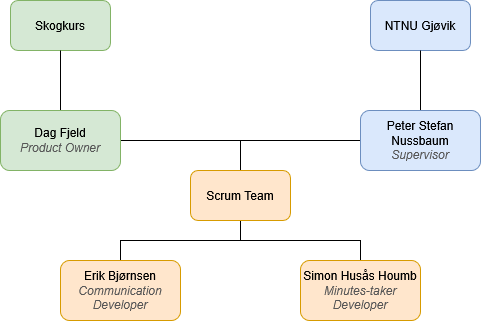
\includegraphics[width=0.75\linewidth]{Images/project_organization.png}
    \caption{Project Organization Diagram}
    \label{fig:prj_org}
\end{figure}

\subsection{Responsibilities \& Roles}
\begin{comment}
    Erik communications
    Simon møtereferent
    Ellers har vi samme responsabilities & roles, 
\end{comment}
\begin{itemize}
    \item Simon Husås Houmb
    \begin{itemize}
        \item Minutes-taker: Tasked with documenting the proceedings for each meeting that is held.
        \item Developer
    \end{itemize}
    \item Erik Bjørnsen
    \begin{itemize}
        \item Communication: Responsible for communicating with Product Owner and Supervisor by mail, etc.
        \item Developer
    \end{itemize}
\end{itemize}

Since both group members share similar backgrounds, responsibilities for specific aspects of the development are not predefined. Instead, they will collaborate on all parts of the project, ensuring that everyone has an opportunity to learn and contribute equally.


\subsection{Routines \& Group Rules}

\subsubsection{General}
\begin{itemize}
    \item The members of the group should work a minimum of 30 hours together per week, preferably on campus.
    \item Decisions that impact the final product should be discussed with the other group member.
    \item All work hours must be recorded with Traggo.
    % TODO: Traggo / Toggl?^
\end{itemize}

\subsubsection{Sickness}
\begin{itemize}
    \item If a group member is sick or for other reasons cannot work, it is still expected that they do their best to get some work done.
    \item If necessary, the other group member is expected to cover for the sick member to ensure a consistent workload.
\end{itemize}

\subsubsection{Meetings}
\begin{itemize}
    \item Meetings with the supervisor will be held every Tuesday at 12:00, unless not necessary or the time is not suitable.
    \item Sprint meetings will be held every Monday, while also having daily scrum meetings.
    \item The proceedings of each meeting will be documented by the minutes-taker.
\end{itemize}

\subsubsection{Communication}
\begin{itemize}
    \item Mutual respect, civility, and humility are required by the group members.
    \item Disagreements are welcome as they are a natural part of working in a team and are vital to any nuanced discussion.
\end{itemize}

\subsubsection{Accountability Measures}
\begin{itemize}
    \item In the event of a conflict, the group will first attempt to resolve it internally. If the issue remains unresolved, a third party may be consulted for assistance. This could include the product owner, the supervisor, or another NTNU professor.
    \item If a group member falls behind in their work, they will be required to use the Easter vacation to catch up.
    \item For minor issues, the group member at fault will be expected to provide a treat (e.g., cinnamon bun, "databrus", beer, "GT") for the other member as a gesture of goodwill. 
\end{itemize}
